\documentclass[letter, 10pt]{article}
\usepackage[utf8]{inputenc}
\usepackage[spanish]{babel}
\usepackage{amsfonts}
\usepackage{amsmath}
% \usepackage[dvips]{graphicx}
\usepackage{url}
\usepackage[top=3cm,bottom=3cm,left=3.5cm,right=3.5cm,footskip=1.5cm,headheight=1.5cm,headsep=.5cm,textheight=3cm]{geometry}
\usepackage[pdftex]{graphicx}



\begin{document}
\title{Inteligencia Artificial \\ \begin{Large}Estado del Arte: Green Vehicle Routing
Problem (GVRP)\end{Large}}
\author{Lucio Fondón Rebolledo}
\date{\today}
\maketitle


%--------------------No borrar esta secci\'on--------------------------------%
\section*{Evaluaci\'on}

\begin{tabular}{ll}
Resumen (5\%): & \underline{\hspace{2cm}} \\
Introducci\'on (5\%):  & \underline{\hspace{2cm}} \\
Definici\'on del Problema (10\%):  & \underline{\hspace{2cm}} \\
Estado del Arte (35\%):  & \underline{\hspace{2cm}} \\
Modelo Matem\'atico (20\%): &  \underline{\hspace{2cm}}\\
Conclusiones (20\%): &  \underline{\hspace{2cm}}\\
Bibliograf\'ia (5\%): & \underline{\hspace{2cm}}\\
 &  \\
\textbf{Nota Final (100\%)}:   & \underline{\hspace{2cm}}
\end{tabular}
%---------------------------------------------------------------------------%
\vspace{2cm}


\begin{abstract}

En este trabajo se realizará un breve estudio del problema de optimización de Green Vehicle Routing Problem (GVRP), el cual consiste en minimizar la distancia recorrida por una flota de vehículos que deben realizar repartos a ciertos clientes predispuestos en posiciones fijas. Ésta flota de vehículos debe iniciar su recorrido en un depósito y al finalizar deben volver a éste. Durante su recorrido, los vehículos pueden detenerse a recargar combustible si es que éstos lo requieren. El GVRP viene del VRP (Vehicle Routing Problem), la diferencia existe en que los vehículos del GVRP utilizan combustibles alternativos para contaminar menos. Lo anterior implica también que existan menos estaciones de combustible, ya que pocos vehículos utilizan combustibles alternativos, por lo que el GVRP es más complejo aún que el VRP.

% Resumen del informe en no m\'as de 10 l\'ineas, donde se sintetice el problema que se trata y sirva para que un lector no involucrado comprenda el objetivo del documento.
\end{abstract}

\section{Introducci\'on}

% Una explicaci\'on breve del contenido del informe, es decir, detalla: Prop\'osito, Estructura del Documento, Descripci\'on (muy breve) del Problema y Motivaci\'on.

Durante las últimas décadas, se ha dado cada vez más importancia al cuidado del medio ambiente en general, donde los gobiernos y empresas se han dedicado a tomar medidas para poder contaminar lo menos posible y atenerse a lo que son las \emph{políticas verdes}, ya que las logísticas que se utilizan hoy en día para la realización de ciertos procesos no son convenientes a largo plazo para el sostenimiento de la calidad del planeta ni el medio ambiente.
\\

Existen una gran cantidad de problemas que se atienen a lo que son las políticas verdes. Uno de los problemas que se estudiará será el de Green Vehicle Routing Problem (GVRP), el cuál consiste en minimizar la distancia recorrida por una flota de vehículos que deben realizar entregas a clientes, partiendo desde un depósito, para luego volver a éste. Durante el trayecto, pueden detenerse a recargar combustible, el cuál es un combustible alternativo que utilizan los vehículos, con el objetivo de minimizar el impacto ambiental producido por éstos.
\\

Primero, se definirá el problema de una manera más coloquial, señalando las principales características del problema, sus restricciones y objetivos, además de mostrar también las principales variantes que existen del problema. Luego, se realizará el \emph{Estado del Arte} del problema, en donde se hará hincapié principalmente en los métodos y algoritmos más utilizados para este tipo de problema, mostrando los distintos \emph{approach} que se han utilizado por investigadores para tratar de resolver este problema.
\\

Después, se presentará un modelo matemático para el problema en cuestión, con el fin de poder acercarse al problema y a su solución desde una perspectiva más matemática y computable, analizando más en profundidad las partes que componen al problema, tales como las variables, su función objetivo, sus restricciones y parámetros.
\\

Finalmente, se mostrarán conclusiones con respecto a todo lo lo presentado anteriormente, especialmente respecto ventajas y desventajas de utilizar o no ciertas técnicas para abordar el problema.


\section{Definici\'on del Problema}
Uno de los problemas combinatoriales de optimización más famosos y estudiados es el Vehicle Routing Problem (VRP), el cual consiste en minimizar la distancia recorrida de una flota de vehículos que deben realizar entregas a un conjunto de clientes, con el objetivo de abaratar costos durante el trayecto.
\\

Mirando desde una perspectiva histórica, el VRP surge a finales de los 50 con los estudios realizados por Dantzig y Ramser \cite{LIN20141118}, en donde ellos indican que el VRP es una generalización del Traveling Salesman Problem (TSP) si es que se le agregan ciertas restricciones a considerar en el contexto del problema del VRP \cite{RePEc:inm:ormnsc:v:6:y:1959:i:1:p:80-91}. Lo anterior es considerado un hincapié inicial para las tantas otras variantes que surgen del problema, hasta finalmente llegar a la variante del GVRP. Ahora, se nombrarán y describirán brevemente las variantes más importantes que surgen de las ideas de Dantzig y Ramser:
\begin{itemize}
    \item \textbf{\emph{Time-dependent VRP}} (TDVRP - 1966): Los primeros trabajos que consideraron esta variante del problema recae en los estudios realizados por Cooke y Halsey. La principal diferencia con VRP es que la distancia entre los puntos a repartir (ya sean clientes, estaciones de  servicio o el depósito) varía dependiendo en qué momento del día se encuentre, ya sea por ejemplo, por condiciones climáticas, horas punta de tráfico, etc. La introducción del TDVRP fue muy relevante para estudios posteriores, en especial los problemas de optimización de redes de tráfico reales  \cite{Cooke1966TheSR}.

    \item \textbf{\emph{Multi-depot VRP}} (MDVRP - 1969): Primeramente estudiado por Tillman en 1969, esta variante contempla que, en vez de que exista un sólo depósito inicial de donde salgan y tengan que volver los vehículos, existan múltiples depósitos de éstos. Este problema se origina principalmente debido a problemas de distribucion de la vida real tales como el reparto de comidas, productos químicos, reparto de productos de una empresa, etc. \cite{doi:10.1287/trsc.3.3.192}
    
    \item \textbf{\emph{Periodic VRP}} (PVRP - 1974): En esta variante, se considera, además de las restricciones ya mencionadas anteriormente del VRP original, que los clientes deben ser visitados en diferentes días dentro de la semana, por lo que el objetivo principal de esta variante es minimizar el costo total de la ruta a lo largo de la planificación de la semana. Beltrami y Bodin en 1974 propusieron algoritmos considerando lo anterior \cite{https://doi.org/10.1002/net.3230040106}.
    
    \item \textbf{\emph{Dynamic VRP}} (DVRP - 1976): En las variantes anteriores, se lidia con información previa acerca de cómo y a donde se deben realizar las entregas, sin embargo, en la vida real no siempre es así. Speidel (1976) y Psaraftis (1980) estudiaron el problema de manera en que la información se va recibiendo en tiempo real, tales como localización de los vehículos y los pedidos de los clientes. Ejemplos de esto son lo servicios de emergencia, servicios de rescate, etc.  \cite{Speidel1976EDPASSISTEDFS} \cite{doi:10.1287/trsc.14.2.130}.
    
    \item \textbf{\emph{VRP with Time windows}} (VRPTW - 1977): Hasta ahora, no se han considerado los tiempos de servicio que se deban cumplir como restricciones. Russell (1977) presentó una heurística para este caso y propuso dos tipos de time windows \cite{doi:10.1287/opre.25.3.517}:
    \begin{itemize}
        \item \emph{Hard Time Windows}: El vehículo debe llegar antes o justo después del tiempo de entrega especificado, y no se permite llegar tarde. Además, si llega antes, el vehículo debe esperar hasta que pase la ventana de tiempo.
        \item \emph{Soft Time Windows}: Las violaciones a las ventanas de tiempo se permiten pero se penalizan a un cierto costo.
    \end{itemize}
\end{itemize}
\\

Teniendo lo anterior en cuenta, se da paso al GVRP (2007) \cite{LIN20141118}. Debido al constante deterioro del medioambiente en el planeta, los gobiernos y empresas comenzaron a adoptar las llamadas logísticas verdes dentro de sus operaciones, es por esto que nace el problema que estudiaremos acá, el Green Vehicle Routing Problem (GVRP), el cual es una variante del VRP en donde los vehículos predispuestos para realizar las entregas a los clientes utilizan un combustible alternativo, con el fin dejar la menor cantidad de contaminación posible en la realización de sus tareas.
\\

El GVRP consiste en realizar una ruta de entregas de una cierta flota de vehículos que parten desde un mismo depósito hacia un conjunto de clientes que se encuentran dispersos geográficamente en un área en particular, para luego volver al mismo depósito inicial, esto con el fin de poder minimizar la distancia recorrida por esta flota de vehículos y así poder también abaratar los costos asociados al trayecto en general. Éstos vehículos pueden realizar paradas en caso de que requieran combustible. Notar que, al utilizar combustible alternativo por ser GVRP, las estaciones serán más limitadas.
\\

Las principales variables a tener en cuenta dentro de este problema serán variables relacionadas a si cierto vehiculo viaja de un punto a otro y variables relacionadas al tiempo de llegada de un vehículo a un punto y el combustible disponible en los vehículos. Además, se tienen que considerar ciertas restricciones que existen en el problema. Los vehículos están restringidos por una cantidad de distancia que pueden recorrer con la cantidad de combustible que almacenan. También, las visitas a un cliente tienen un tiempo de servicio asociado. Cuando un vehículo requiera llenarse de combustible, también tomará un tiempo de recarga de combustible. Además, los vehículos están restringidos a un tiempo de servicio que no pueden sobrepasar antes de volver al depósito. Por otro lado, cada cliente debe visitarse una sola vez por un solo vehículo. Por último, se tomará en consideración que no existe un límite de vehículos disponibles en la flota y que la velocidad de éstos es constante.

% Explicaci\'on del problema que se va a estudiar, en qu\'e consiste, cu\'ales son sus variables , restricciones y objetivo(s) de manera general (en palabras, no una formulaci\'on matem\'atica). Debe entenderse claramente el problema y qu\'e busca resolver.
% Explicar si existen problemas relacionados.
% Destacar, si existen, las variantes m\'as conocidas.\\
% Redactar en tercera persona, sin faltas de ortograf\'ia y referenciar correctamente sus fuentes mediante el comando  \verb+\cite{ }+. Por ejemplo, para hacer referencia al art\'iculo de algoritmos h\'ibridos para problemas de satisfacci\'on 
%  de restricciones~\cite{MOGHDANI2021123691}.

\section{Estado del Arte}

Como se mencionó anteriormente, el GVRP es una variante del problema original VRP. El Vehicle Routing Problem fue introducido por primera ver por Dantzig y Ramser (1959), y mencionan que el problema viene directamente del conocido Traveling Salesman Problem (TSP) \cite{RePEc:inm:ormnsc:v:6:y:1959:i:1:p:80-91}. El problema lo describen como un \emph{routing problem}, en donde camiones con gasolina debían repartir a ciertas estaciones de servicio geográficamente esparcidas en un espacio en particular. Sin embargo, se dieron cuenta que si la cantidad de estaciones de servicio aumentaban, entonces las opciones de ruta crecían considerablemente y tratar de encontrar una solución óptima se hacía una tarea muy difícil de realizar. Por lo anterior, propusieron un algoritmo basado en programación lineal entera, para poder obtener una solución cercana a la óptima. A esta variante inicial de VRP se le llamó \emph{Capacitated VRP} \cite{LIN20141118}.
\\

A lo largo de los años, y junto con todas las resoluciones de las variantes del problema de VRP, se muestra a continuación los métodos y algoritmos utilizados en general para la resolución de éstos.\\

\begin{figure}[h]
    \centering
    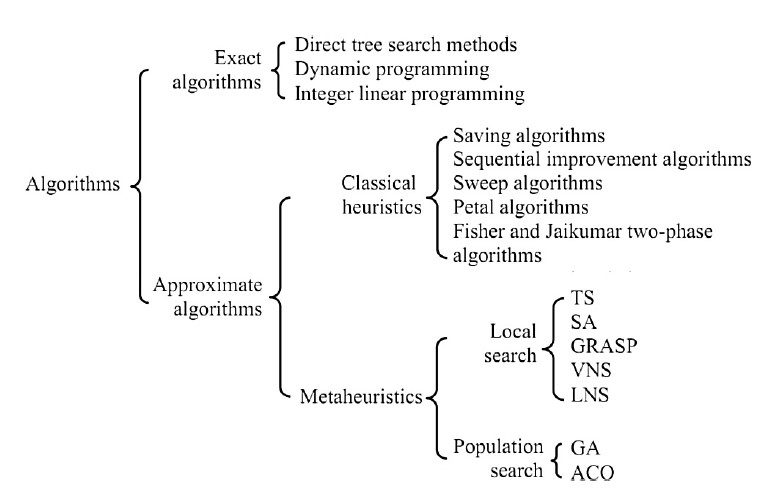
\includegraphics[width=12cm]{AlgoritmosVRP.jpg}
    \caption{Métodos más utilizados para VRP  \cite{LIN20141118}}
    \label{fig:figura1}
\end{figure}

Se detallarán ahora brevemente algunos de los métodos utilizados más importantes para la resolución del VRP y sus variantes mostradas en la imagen anterior:

\subsection{Algoritmos Exactos}
Dentro de los algoritmos exactos podemos hallar 3 métodos distintos que se han utilizado a lo largo de la historia para resolver los problemas de VRP:
\begin{itemize}
  \item \textbf{\emph{Programación Lineal Entera}}: Es sabido que la programación lineal entera ha sido uno de los primeros métodos en general para la resolución de problemas en donde se debían minimizar o maximizar una cierta variable para algún problema. En el caso de los problemas de VRP no es distinto; Dantzig y Ramser, los primeros en presentar el problema de VRP, utilizaron de hecho una estrategia usando programación lineal entera \cite{RePEc:inm:ormnsc:v:6:y:1959:i:1:p:80-91}. También, junto con la programación lineal entera, se utilizaron métodos de \emph{set partitioning} y \emph{generación de columnas} propuestas por Balinski y Quandt \cite{BALINSKIQUANDT}. Sin embargo, las soluciones utilizando programación lineal entera, por lo general, no pueden escalar a problemas dentro de la vida real, específicamente por la gran cantidad de variables binarias que se generan, por lo que se hace muy difícil computacionalmente llegar a soluciones exactas óptimas \cite{LAPORTE1992345}.
  
    \item \textbf{\emph{Programación Dinámica}}: Otro approach utilizando métodos con algoritmos exactos es con el uso de programación dinámica, en donde, generalmente, se utiliza el famoso método de recursión para la resolución del problema. Eilon, Watson-Gandy y Christofides (1971) fueron los primeros en proponer algoritmos de programación dinámica para la resolución de un VRP \cite{Burrows1972DistributionMM}. Éstos algoritmos tuvieron un par de mejoras con una relajación del estado-espacio propuestas por Christofides, Mingozzi y Toth, donde se concluyó que con instancias que contenían de 10 a 25 vértices podían resolverse teniendo la solución óptima \cite{CHRISTOFIDESNICOSMINGOZZITOTH}.
    
    \item \textbf{\emph{Métodos basados en búsquedas con árboles}}: Un método interesante propuesto para resolver problemas de VRP son los basados en búsquedas de árboles.  Laporte, Nobert y Taillefer lograron obtener resultados muy prometedores con la contraparte de la programación linea y programación dinámica, donde se utilizó el conocido método de \emph{branch and bound} en conjunto con métodos de resolución para problemas de asignación, llegando a resolver instancias del problema con más de 100 vértices involucrados óptimamente \cite{LAPORTE1987857}.

\end{itemize}

\subsection{Algoritmos Aproximados}
En los algoritmos aproximados que se han utilizado a lo largo de la historia para resolver instancias del VRP y sus variantes, podemos dividirlos en dos categorías: las \emph{heurísticas clásicas} y las \emph{metaheurísticas}. Dentro de las heurísticas clásicas podemos destacar los siguientes métodos utilizados:

\begin{itemize}
    \item \textbf{\emph{Algoritmos de Ahorro}}: Clarke y Wrigth (1964) propusieron una heurística clásica para el VRP, y probablemente sea la más conocida para este tipo de problema, y generalmente se utiliza cuando el número de vehículos son una variable de decisión. Éste método produjo soluciones cuyos valores se encuentran un $6.71\%$ por sobre las que se conocen \cite{CLASSICHEURISTICS}.
    
    \item \textbf{\emph{Algoritmos de Barrido}}: El algoritmo de barrido se aplica a instancias planares del VRP, en donde la ruta del vehículo se obtiene dentro un clúster en específico utilizando la resolución de un TSP, de tal manera que se inicializa una ruta (eligiendo a algún vehículo), se construye una ruta (clusterizando) y luego se optimiza dicha ruta con TSP. Una generalización de éste algoritmo es el Algoritmo de Pétalos, que combina lo anterior dicho con resolver también un problema de set partitioning. \cite{CLASSICHEURISTICS}.
    
    \item \textbf{\emph{Algoritmo de Fisher y Jaikumar}}: Fisher y Jaikuman propusieron un algoritmo de dos fases, en donde primero crean clústers de los clientes a donde se deben repartir los productos resolviend un problema de asignación generalizada, y luego poder determinar la ruta óptima con un algoritmo de TSP. Sin embargo, quedaron ciertas dudas acerca del rendimiento de este algoritmo debido a que no se utilizaron correctas reglas de truncación o redondeo en los resultados finales de las soluciones, por lo que no pueden ser correctamente verificadas \cite{GUIDETOVRP}.
\end{itemize}
Por otro lado, dentro de las metaheurísticas, podemos dividirlos en dos ramas:
\begin{itemize}
    \item \textbf{\emph{Técnicas de Búsqueda Local}}: Éstas técnicas se basan en explotar el espacio de soluciones al moverse iterativamente desde una solución a otra más prometedora dentro de su vecindario \cite{LIN20141118}. Dentro del VRP, el \emph{Tabu Search} (TS) y \emph{Simulated Annealing} (SA) han sido de las metaheurísitcas que han dado buenos resultados para las instancias del VRP, Osman lo concluye así en sus estudios \cite{OSMAN}. 
    \item \textbf{\emph{Técnicas basadas en Población}}: Los métodos basados en población mantiene unn \emph{pool} de soluciones prometedoras, y se actualiza éste pool a medida que encuentra otras mejores. En esta categoría se encuentran los \emph{Genetic Algorithms} (GA) y los \emph{Ant Colony Optimization} (ACO). Se ha demostrado que para el GVRP, utilizando un approach de algoritmo genético híbrido se pueden obtener spluciones sustancialmente mejores que utilizando ACO y branch and cut (B\&C) \cite{10.1007/978-3-642-13803-4_15}.
\end{itemize}

Las publicaciones en los últimos años acerca de resoluciones y métodos nuevos para el GVRP y variantes del VRP siguen creciendo. Sin embargo, los estudios que existen son limitados principalmente debido a que involucra muchos factores que son complicados hoy en día, tales como energía e impacto ambiental, polución, planificamiento urbano, etc.
\\

En general, los problemas de GVRP que se analizan hoy en día tienen que ver con aquellos que tienen comportamiento \emph{no determinista}, es decir, \textbf{VRP con incertidumbres}. Algunos ejemplos son los VRP con servicio de tiempo estocástico, demanda de clientes estocástica y tiempo de viaje estocástico, los cuáles se asemejan más a la realidad de estos problemas, pero a su vez son tremendanmente más complejos de resolver \cite{LIN20141118}.

% La informaci\'on que describen en este punto se basa en los estudios realizados con antelaci\'on respecto al tema.
% Lo m\'as importante que se ha hecho hasta ahora con relaci\'on al problema. Deber\'ia responder preguntas como las siguientes:
% ?`cu\'ando surge?, ?`qu\'e m\'etodos se han usado para resolverlo?, ?`cu\'ales son los mejores algoritmos que se han creado hasta
% la fecha?, ?`qu\'e representaciones han tenido los mejores resultados?, ?`cu\'al es la tendencia actual para resolver el problema?, tipos de movimientos, heur\'isticas, m\'etodos completos, tendencias, etc... Puede incluir gr\'aficos comparativos o explicativos.\\



\section{Modelo Matem\'atico}

Ahora, se presentará un modelo matemático para el problema del GVRP, el cuál se define como un grafo completo no dirigido $G = (V,E)$. En este caso, usaremos el modelo planteado por Erdoğan y Miller-Hooks \cite{ERDOGANMILLERHOOKS}. Este estudio fue el primero en introducir lo que son los \emph{Alternative Fuel-powered Vehicles} (AFV) en el problema del GVRP, por lo que toma en cuenta lo que necesitamos para poder resolver el problema utilizando políticas verdes y obtener una solución óptima en minimización de distancia recorrida y costos de entrega. Cabe destacar que este modelo es formulado en base a programación lineal entera mixta.

\subsection{Parámetros}
\begin{itemize}
    \item $I$: Conjunto de vértices de los clientes.
    \item $F$: Conjunto de vértices de las estaciones de recarga.
    \item $v_0$: Depósito inicial (punto de partida y llegada de los vehículos).
    \item $V$: Conjunto de todos los vértices (Notar que $V = \{v_0\} \cup I \cup F$).
    \item $d_{ij}$: Distancia desde el vértice $i$ hasta el vértice $j$.
    \item $p_i$: Tiempo de servicio que toma en el vértice $i$ (Si $i \in I$, entonces corresponde al tiempo de servicio al cliente. Si $i \in F$, entonces corresponde al tiempo de recarga de combustible en una estación).
    \item $Q$: Capacidad del tanque de combustible del vehículo.  (El valor del combustible restante de un vehículo toma el valor de $Q$ cada vez que se recargue combustible).
    \item $r$: Velocidad de consumo de combutible del vehículo.
\end{itemize}

\subsection{Variables}
\begin{itemize}
    \item     $x_{ij} = \left\{
        \begin{array}{ll}
            1 & \quad \text{Si el vehículo viaja desde el vértice $i$ hasta el vértice $j$} \\
            0 & \quad \text{Caso contrario}
        \end{array}
    \right.$
    \item $y_j$ = Nivel de combustible del vehículo restante al llegar al vértice $j$.
    \item $\tau_j$ = Tiempo de arribo de un vehículo al vértice $j$. Se inicializa en $0$ partiendo desde $v_0$.
\end{itemize}

\subsection{Función objetivo}
\begin{align}
    \min F:
    & \sum_{\substack{(i,j)\in V\\ i \neq j}} d_{ij} x_{ij}
\end{align}
\begin{center}
    Ecuación 1: Función objetivo asociada al problema del GVRP propuesta por Erdoğan y Miller-Hooks. Busca minimizar la distancia total recorrida por un vehículo de la flota.
\end{center}

\subsection{Restricciones}
\begin{align}
    \sum_{\substack{j\in V\\ j \neq i}} x_{ij} = 1, & \quad \forall i \in I
\end{align}

\begin{center}
    Ecuación 2: Maneja que cada vértice perteneciente al conjunto de los clientes tenga un solo sucesor, ya sea una estación de recarga, otro cliente o el depósito inicial $v_0$.
\end{center}

\begin{align}
    \sum_{\substack{j\in V\\ j \neq i}} x_{ij} \leq 1, & \quad \forall i \in F
\end{align}

\begin{center}
    Ecuación 3: Se asegura que cada vértice perteneciente al conjunto de las estaciones de recarga tenga a lo más un sucesor, ya sea una estación de recarga, otro cliente o el depósito inicial $v_0$.
\end{center}

\begin{align}
    \sum_{\substack{i\in V\\ j \neq i}} x_{ji} - \sum_{\substack{i\in V\\ j \neq i}} x_{ij} = 0, & \quad \forall j \in V
\end{align}

\begin{center}
    Ecuación 4: Esta restricción se asegura que el número de llegadas a cada vértice perteneciente a $V$ sea el mismo que el número de salidas.
\end{center}


% \begin{align}
%     \sum_{\substack{j\in V \text{\textbackslash} \{0\}}} x_{0j} \leq m
% \end{align}

% \begin{align}
%     \sum_{\substack{j\in V \text{\textbackslash} \{0\}}} x_{j0} \leq m
% \end{align}

\begin{align}
    \tau_j \geq \tau_i + (t_{ij} - p_j)x_{ij} - T_{\text{max}}(1 - x_{ij}), & \quad \forall i \in V, \forall j \in V \text{\textbackslash}\{0\}, i \neq j
\end{align}

\begin{center}
    Ecuación 5: Esta restricción es necesaria para tener registro del tiempo en el que cada vértice $i$ es visitado y el tiempo en que le toma llegar al vértice $j$, para así poder prevenir subrutas.
\end{center}


\begin{align}
    0 \leq \tau_0 \leq T_{\text{max}}
\end{align}

\begin{center}
    Ecuación 6: Se asegura de que cada vehículo no exceda el tiempo máximo $T_{\text{max}}$ de tiempo de llegada de vuelta al depósito, especificando el tiempo con el que parte el vehículo desde el depósito $v_0$.
\end{center}

\begin{align}
    t_{0j} \leq \tau_j \leq T_{\text{max}} - (t_{j0} + p_j), \quad \forall j \in V \text{\textbackslash}\{0\}
\end{align}

\begin{center}
    Ecuación 7: Se asegura que cada vehículo termine la ruta en el tiempo máximo $T_{\text{max}}$.
\end{center}

\begin{align}
    y_j \leq y_i - r \cdot d_{ij}x_{ij} + Q(1 - x_{ij}), \quad \forall j \in I \text{ y } i \in V, i \neq j
\end{align}

\begin{center}
    Ecuación 8: Se encarga de reducir el nivel de carga de combustible del vehículo que llega a un vértice $j$, considerando la distancia recorrida desde $i$ hasta $j$ y la velocidad $r$ a la que va el vehículo.
\end{center}

\begin{align}
    y_j = Q, & \quad \forall j \in F
\end{align}

\begin{center}
    Ecuación 9: Encargada de setear nuevamente el nivel de combustble de un vehículo al visitar a una estación de recarga.
\end{center}

\begin{align}
    y_j \geq \min \{r \cdot d_{j0}, r(d_{jl} + d_{l0})\}
\end{align}

\begin{center}
    Ecuación 10: Garantiza que el vehículo cuente con el combustible necesario para poder volver al depósito o a una estación de recarga.
\end{center}

\subsection{Naturaleza de las Variables}
\begin{itemize}
    \item $x_{ij}$: Variable de decisión booleana. $x \in \{0,1\}$
    \item $\tau_j, y_j$: Variables tipo entero. $\tau_j, y_j \in \mathbb{Z}$
\end{itemize}


% Uno o m\'as modelos matem\'aticos para el problema, idealmente indicando el espacio de b\'usqueda para cada uno. Cada modelo debe estar correctamente referenciado, adem\'as no debe ser una imagen extraida. Tambi\'en deben explicarse en detalle cada una de las partes, mostrando claramente la funci\'on a maximizar/minimizar, variables y restricciones. Tanto las f\'ormulas como las explicaciones deben ser consistentes.

\section{Conclusiones}
Los tipos de problemas de optimización de VRP se han vuelto muy importantes para poder mejorar los procesos de reparto de suministros a clientes, en donde se busca minimizar los costos asociados y sacarle el máximo provecho a los vehículos que se utilizan. A lo largo del escrito, se vieron distintos tipos de métodos, algoritmos y técnicas que se utilizan para poder resolver estos problemas.
Dependiendo del tipo de variante del VRP que se esté tratando de resolver se utilizaron distintos métodos, pero por lo general, los algoritmos de programación lineal entera y programación lineal entera mixta son los que predominan principalmente por su simpleza en la formulación de éstos, no necesariamente siendo los que obtienen mejores resultados. Por otro lado, los algoritmos aproximados suelen tener mejores resultados que los algoritmos exactos debido a que buscan soluciones cercanas las óptimas con un margen de error muy pequeño, siendo las técnicas de búsqueda local, tales como Tabu Search (TS) y Simulated Annealing (SA) las que han llevado a obtener mejores resultados, aunque también realizando algoritmos híbridos se ha podido llegar a buenos resultados. Aunque se hayan realizado bastantes estudios en los problemas de VRP en general, el problema de GVRP es relativamente nuevo debido a la preocupación de hoy en día por minimizar la polución y tratar de realizar procesos industriales utilizando políticas verdes. Si bien se efectúan continuamente estudios sobre como abordar mejor el GVRP, para las investigaciones futuras se está tornando interesante el estudio de problemas de GVRP de carácter estocástico, por lo que probablemente las investigaciones venideras harán un buen hincacapié en ese lado para poder seguir profundizando más la resolución del problema.
% Conclusiones RELEVANTES del estudio realizado. Deber\'ia responder a las preguntas: ?`todas las t\'ecnicas resuelven el mismo problema o hay algunas diferencias?, ?`En qu\'e se parecen o difieren las t\'ecnicas en el contexto del problema?, ?`qu\'e limitaciones tienen?, ?`qu\'e t\'ecnicas o estrategias son las m\'as prometedoras?, ?`existe trabajo futuro por realizar?, ?`qu\'e ideas usted propone como lineamientos para continuar con investigaciones futuras?


\section{Bibliograf\'ia}
\bibliographystyle{plain}
\bibliography{Referencias}

\end{document} 
